\documentclass[12pt,a4paper]{article}

\usepackage[utf8]{inputenc}
\usepackage[T1]{fontenc}
\usepackage{amsmath,amssymb,amsfonts}
\usepackage{mathtools}
\usepackage{booktabs}
\usepackage{array}
\usepackage{graphicx}
\usepackage{xcolor}
\usepackage{hyperref}
\usepackage[margin=2.5cm]{geometry}
\usepackage{caption}
\usepackage{enumitem}
\usepackage{float}
\usepackage{natbib}
\usepackage{tikz}
\usetikzlibrary{positioning,arrows.meta,3d}

\hypersetup{
  colorlinks=true,
  linkcolor=blue!60!black,
  citecolor=blue!60!black,
  urlcolor=blue!60!black
}

\newcommand{\circlette}{\textit{circlette}}
\newcommand{\circlettes}{\textit{circlettes}}
\newcommand{\bitstr}[1]{\texttt{#1}}

\title{\textbf{It from Bit, Revisited:}\\[6pt]
Standard Model Fermions as Codewords\\of a Holographic Error-Correcting Code,\\
with Forces, Mass, and Gravity\\as Information Flow on the Lattice}

\author{
  D.~[Author]\footnote{Email: \texttt{[email]}}\\[4pt]
  \textit{Neuro-Symbolic Ltd}\\
  \textit{United Kingdom}
}

\date{February 2026}

\begin{document}

\maketitle

% ============================================================
\begin{abstract}
We propose that the fermion spectrum of the Standard Model is the set of valid codewords of a quantum error-correcting code defined on a holographic boundary surface. Each fundamental fermion is encoded as an oriented ring of 8 bits---a \emph{\circlette{}}---where matter and antimatter are distinguished by reading direction. Four local constraints, none spanning more than three adjacent bits on the ring, select exactly 45 valid matter states from 256 possibilities (90 total including antimatter). The ring partitions into three sectors---generation, colour, and electroweak---connected by a bridge bit, mirroring the gauge group factorisation $SU(3) \times SU(2) \times U(1)$ directly onto a topological structure.

Starting from this encoding, we develop a complete dynamical and geometric framework. Colour confinement reduces to XOR closure. The CKM mixing hierarchy is reproduced by a weighted Hamming metric on the generation bits. Gauge bosons are formalised as specific bit-manipulation operators: gluons as colour permutation matrices, the $W$ boson as a conditional chirality-gated flip. Particle mass emerges from the circulation frequency of ring patterns on the lattice. Grand unification corresponds to the bridge bit entering quantum superposition at high energies. The Heisenberg uncertainty principle follows from the Bekenstein information bound as a hard limit on computational bandwidth.

The deepest result concerns gravity. We define a Fisher information metric on the lattice's statistical states and show that it provides a quantitative bridge from discrete lattice tension to the Riemannian geometry of general relativity. An information action principle---the integral of Fisher arc-length along a path---unifies three pillars: the geodesic equation (gravity), the Feynman path integral (quantum mechanics), and Noether's theorem (conservation laws) as three aspects of a single variational structure. Momentum, energy, and angular momentum emerge as Noether charges of the update rule's symmetries. The stress-energy tensor is identified with the gradient of bit-density. The cosmological constant emerges as the information floor---the minimum bit density for causal connectivity. The equivalence of inertial and gravitational mass becomes a mathematical identity: both measure the same lattice bandwidth cost. A novel prediction---lattice-induced decoherence---arises from the discreteness of the information substrate, producing mass-dependent and gravity-dependent coherence loss distinct from environmental decoherence.

The framework traces a trajectory from \emph{It from Bit} (static encoding) through \emph{It from Computation} (dynamic operators and update rules) to \emph{It from Geometry} (information-geometric emergence of general relativity), offering a unified computational architecture grounded in Wheeler's programme, the holographic principle, and 't~Hooft's cellular automaton interpretation.
\end{abstract}

\vspace{1em}
\noindent\textbf{Keywords:} holographic principle, error-correcting codes, emergent gravity, Fisher information metric, information geometry, information action, lattice-induced decoherence, CKM matrix, grand unification, cellular automaton, Feynman path integral

% ============================================================
% PART I: IT FROM BIT — THE ENCODING
% ============================================================

\part*{Part I: It from Bit}
\addcontentsline{toc}{part}{Part I: It from Bit}

\section{Introduction}
\label{sec:intro}

In 1990, John Archibald Wheeler proposed that the physical world might ultimately be built from information---that every particle, every field, every spacetime event derives its existence from binary choices, from bits~\citep{Wheeler1990}. He called this vision ``It from Bit.'' Three decades later, the holographic principle~\citep{Bekenstein1973,Susskind1995}, the ER=EPR conjecture~\citep{Maldacena2013}, and 't~Hooft's cellular automaton interpretation~\citep{tHooft2016} have all provided evidence that this vision may be correct. Yet a concrete realisation has been elusive: which bits? What code? What rules?

This paper proposes specific answers. We show that:
\begin{enumerate}[nosep]
  \item The 90 fundamental fermions of the Standard Model (45 matter + 45 antimatter) can be exactly represented as the valid codewords of an 8-bit error-correcting code.
  \item The bits arrange naturally on an oriented ring (a \circlette{}), with four local rules selecting the valid states.
  \item The ring's topology mirrors the gauge group factorisation $SU(3)_C \times SU(2)_L \times U(1)_Y$.
  \item Colour confinement, the CKM matrix, and particle lifetimes all have natural interpretations within the code.
  \item The four fundamental forces arise as specific bit-manipulation operators on the ring.
  \item Mass emerges from the circulation frequency of ring patterns on a holographic lattice.
  \item Grand unification corresponds to a ring bit entering quantum superposition.
  \item The uncertainty principle is a consequence of finite information capacity.
  \item General relativity emerges from the Fisher information geometry of the lattice's statistical states.
\end{enumerate}

Rather than proposing a general principle and searching for consequences, we start from the known particle spectrum and ask: what is the simplest binary encoding that reproduces it exactly, and do the structural properties of that encoding correspond to known physics? The answer, we find, is surprisingly rich.


% ============================================================
\section{The Encoding}
\label{sec:encoding}

A fermion in the Standard Model is specified by a small number of discrete quantum numbers. We encode these as an 8-bit string with the layout shown in Table~\ref{tab:encoding}. An additional bit---the matter/antimatter distinction---is encoded not as a ninth bit but as the \emph{orientation} of the ring (Section~\ref{sec:ring}).

\begin{table}[H]
\centering
\caption{The 8-bit fermion encoding.}
\label{tab:encoding}
\begin{tabular}{c l l}
\toprule
\textbf{Bit(s)} & \textbf{Field} & \textbf{Values} \\
\midrule
$b_1$--$b_2$ & Generation ($G_0, G_1$) & $00$ = 1st, $01$ = 2nd, $10$ = 3rd, $11$ = forbidden \\
$b_3$ & Lepton/Quark ($LQ$) & $0$ = lepton, $1$ = quark \\
$b_4$--$b_5$ & Colour ($C_0, C_1$) & $00$ = white, $01$ = red, $10$ = green, $11$ = blue \\
$b_6$ & Isospin type ($I_3$) & $0$ = up-type, $1$ = down-type \\
$b_7$ & Chirality ($\chi$) & $0$ = left-handed, $1$ = right-handed \\
$b_8$ & Weak participation ($W$) & $0$ = doublet, $1$ = singlet \\
\bottomrule
\end{tabular}
\end{table}

Eight bits yield $2^8 = 256$ possible states. Of these, exactly 45 satisfy all physical consistency constraints---the parity checks of our code. These 45 states are the fundamental fermions of the Standard Model for matter: 15 states per generation (counting colour and chirality variants), times 3 generations. Including antimatter (Section~\ref{sec:ring}) gives the full 90.

The electric charge of any codeword is derivable from two bits. For quarks ($b_3 = 1$): $Q = +\tfrac{2}{3}$ if $b_6 = 0$ (up-type), $Q = -\tfrac{1}{3}$ if $b_6 = 1$ (down-type). For leptons ($b_3 = 0$): $Q = 0$ if $b_6 = 0$ (neutrino), $Q = -1$ if $b_6 = 1$ (charged lepton). More concisely:
\begin{equation}
Q = b_3 \cdot \tfrac{1}{3}(1 - 2b_6) + (1 - b_3)(-b_6)
\label{eq:charge}
\end{equation}
The fact that charge reduces to a function of two bits ($b_3$ and $b_6$) is itself notable: it suggests that electric charge is not a continuous parameter but a derived binary property.


% ============================================================
\section{The Parity Checks}
\label{sec:parity}

Six constraints act as the parity check matrix of the code. A bit string is a valid codeword---a real particle---if and only if it satisfies all six:

\begin{enumerate}[label=\textbf{C\arabic*:},leftmargin=2em]
  \item \textbf{Colour--lepton exclusion.} If $b_3 = 0$ (lepton), then $b_4 = b_5 = 0$ (colourless). Leptons do not carry colour charge.
  
  \item \textbf{Quark colour requirement.} If $b_3 = 1$ (quark), then $(b_4, b_5) \neq (0,0)$. Quarks must carry colour.
  
  \item \textbf{Chirality--weak coupling.} $b_7 = b_8$: chirality equals weak participation. Left-handed particles form $SU(2)_L$ doublets; right-handed particles are singlets.
  
  \item \textbf{Generation bound.} $(b_1, b_2) \neq (1,1)$. There are exactly three generations.
  
  \item \textbf{No right-handed neutrino.} Not $(b_3 = 0$ and $b_6 = 0$ and $b_7 = 1)$. There is no right-handed neutrino in the Standard Model.
  
  \item \textbf{Antimatter consistency.} (Encoded by ring orientation rather than bit value---see Section~\ref{sec:ring}.)
\end{enumerate}

Applied to all $256$ possible 8-bit strings, these constraints select exactly 45 valid matter codewords: the 15 first-generation fermions (Table~\ref{tab:codewords}), replicated identically for generations 2 ($b_1 b_2 = 01$) and 3 ($b_1 b_2 = 10$).


% ============================================================
\section{The Codewords}
\label{sec:codewords}

\begin{table}[H]
\centering
\caption{First-generation matter codewords (15 states). $\chi$: chirality; Col: colour; Bits: $b_1 b_2 b_3 b_4 b_5 b_6 b_7 b_8$.}
\label{tab:codewords}
\begin{tabular}{l c c c}
\toprule
\textbf{Particle} & $\boldsymbol{\chi}$ & \textbf{Col} & \textbf{Codeword} \\
\midrule
$\nu_e$ (neutrino) & L & --- & \bitstr{00\,0\,00\,0\,00} \\
$e^-$ (electron) & L & --- & \bitstr{00\,0\,00\,1\,00} \\
$e^-$ (electron) & R & --- & \bitstr{00\,0\,00\,1\,11} \\
\midrule
$u$ (up quark) & L & r & \bitstr{00\,1\,01\,0\,00} \\
$u$ (up quark) & L & g & \bitstr{00\,1\,10\,0\,00} \\
$u$ (up quark) & L & b & \bitstr{00\,1\,11\,0\,00} \\
$u$ (up quark) & R & r & \bitstr{00\,1\,01\,0\,11} \\
$u$ (up quark) & R & g & \bitstr{00\,1\,10\,0\,11} \\
$u$ (up quark) & R & b & \bitstr{00\,1\,11\,0\,11} \\
\midrule
$d$ (down quark) & L & r & \bitstr{00\,1\,01\,1\,00} \\
$d$ (down quark) & L & g & \bitstr{00\,1\,10\,1\,00} \\
$d$ (down quark) & L & b & \bitstr{00\,1\,11\,1\,00} \\
$d$ (down quark) & R & r & \bitstr{00\,1\,01\,1\,11} \\
$d$ (down quark) & R & g & \bitstr{00\,1\,10\,1\,11} \\
$d$ (down quark) & R & b & \bitstr{00\,1\,11\,1\,11} \\
\bottomrule
\end{tabular}
\end{table}

All 15 first-generation states have zero parity violations. They are exact codewords. The pattern repeats identically for generations 2 and 3 (with $b_1 b_2$ set to $01$ and $10$ respectively). This is what we mean by ``stable'' in the code-theoretic sense: these patterns satisfy all parity checks and persist indefinitely.


% ============================================================
\section{Colour as XOR}
\label{sec:colour}

The colour charge encoding has a remarkable algebraic property. Using the assignment $r = 01$, $g = 10$, $b = 11$, and white $= 00$:
\begin{align}
r \oplus g \oplus b &= 01 \oplus 10 \oplus 11 = 00 = \text{white} \label{eq:baryon}\\
r \oplus \bar{r} &= 01 \oplus 01 = 00 = \text{white} \label{eq:meson}
\end{align}

A baryon (three quarks) is colour-confined because the XOR of its three colour bit-pairs is $00$ (Eq.~\ref{eq:baryon}). A meson (quark--antiquark) is colour-confined because a colour XORed with itself yields $00$ (Eq.~\ref{eq:meson}). The rule that free particles must be colourless is the statement that the colour bits of any observable composite must XOR to zero.

This is not merely a notational convenience. XOR is the addition operation in $\mathbb{F}_2^2$, the two-dimensional vector space over the field with two elements. That the fundamental non-abelian gauge symmetry of the strong force reduces to $\mathbb{F}_2^2$ closure in this encoding suggests that the encoding is not arbitrary but reflects the underlying information structure.


% ============================================================
\section{The CKM Matrix as Hamming Distance}
\label{sec:ckm_basic}

The Cabibbo--Kobayashi--Maskawa (CKM) matrix describes the probability amplitudes for quark flavour-changing weak decays~\citep{PDG2024}. Its entries are free parameters in the Standard Model---measured, not derived. In our encoding, these entries correlate with the Hamming distance between generation bit-pairs.

\begin{table}[H]
\centering
\caption{CKM matrix elements and generation bit-flip distances.}
\label{tab:ckm}
\begin{tabular}{l c c r l}
\toprule
\textbf{Element} & \textbf{Gen bits} & $\boldsymbol{d_H}$ & $\boldsymbol{|V_{ij}|^2}$ & \textbf{Category} \\
\midrule
$|V_{ud}|^2$ & $00 \to 00$ & 0 & $0.974$ & Same generation \\
$|V_{us}|^2$ & $01 \to 00$ & 1 & $0.053$ & Adjacent \\
$|V_{ub}|^2$ & $10 \to 00$ & 1 & $1.3 \times 10^{-5}$ & Distant \\
\midrule
$|V_{cd}|^2$ & $00 \to 01$ & 1 & $0.053$ & Adjacent \\
$|V_{cs}|^2$ & $01 \to 01$ & 0 & $0.974$ & Same generation \\
$|V_{cb}|^2$ & $10 \to 01$ & 2 & $1.7 \times 10^{-3}$ & Adjacent \\
\midrule
$|V_{td}|^2$ & $00 \to 10$ & 1 & $7.4 \times 10^{-5}$ & Distant \\
$|V_{ts}|^2$ & $01 \to 10$ & 2 & $1.6 \times 10^{-3}$ & Adjacent \\
$|V_{tb}|^2$ & $10 \to 10$ & 0 & $0.999$ & Same generation \\
\bottomrule
\end{tabular}
\end{table}

The pattern is clear: each additional bit flip costs approximately 1.5--2.5 orders of magnitude in transition probability. This is the behaviour of an error-correcting code, where transitions requiring more bit changes are exponentially suppressed. However, the standard Hamming distance fails to distinguish $|V_{ub}|^2$ from $|V_{ts}|^2$ despite both involving one-bit transitions. We refine this in Section~\ref{sec:ckm_weighted}.


% ============================================================
\section{Generation Distance and Particle Lifetimes}
\label{sec:lifetimes}

If higher-generation particles are ``near-codewords''---patterns that satisfy the structural parity checks but violate a generation stability condition---then their lifetime should correlate with the number of such violations.

\begin{table}[H]
\centering
\caption{Generation parity violations and particle lifetimes.}
\label{tab:lifetime}
\begin{tabular}{l c c c r}
\toprule
\textbf{Particle} & \textbf{Gen} & \textbf{PV} & $\boldsymbol{\tau}$ \textbf{(s)} & $\boldsymbol{\log_{10}\tau}$ \\
\midrule
Muon ($\mu$) & 2 & 1 & $2.2 \times 10^{-6}$ & $-5.7$ \\
Strange ($s$) & 2 & 1 & $1.2 \times 10^{-8}$ & $-7.9$ \\
Charm ($c$) & 2 & 1 & $1.0 \times 10^{-12}$ & $-12.0$ \\
\midrule
Tau ($\tau$) & 3 & 2 & $2.9 \times 10^{-13}$ & $-12.5$ \\
Bottom ($b$) & 3 & 2 & $1.3 \times 10^{-12}$ & $-11.9$ \\
Top ($t$) & 3 & 2 & $5.0 \times 10^{-25}$ & $-24.3$ \\
\bottomrule
\end{tabular}
\end{table}

For each particle type---charged lepton, down-type quark, up-type quark---moving from generation 2 to generation 3 (adding one parity violation) consistently reduces the lifetime by many orders of magnitude, substantially exceeding what can be attributed to the mass increase alone. This is consistent with the error-correcting code interpretation: codewords at greater Hamming distance from the stable first-generation patterns are less stable.


% ============================================================
\section{The Ring Topology}
\label{sec:ring}

The parity checks (Section~\ref{sec:parity}) involve different subsets of bits. Do they simplify when the bits are arranged geometrically? We searched all 5,040 distinct circular orderings of the 8 bits and evaluated the \emph{locality} of each constraint---whether the bits it involves are adjacent on the ring.

Of 5,040 orderings, exactly 48 achieve \emph{perfect locality}: all constraints reduce to nearest-neighbour or next-nearest-neighbour checks on the ring. The 8 optimal orderings (locality score 8) all share the same abstract structure, up to colour-bit swap ($C_0 \leftrightarrow C_1$) and ring reversal:

\begin{equation}
\underbrace{G_0 \;-\; G_1}_{\text{generation}} \;-\; \underbrace{C_0 \;-\; C_1}_{\text{colour}} \;-\; \underset{\text{bridge}}{LQ} \;-\; \underbrace{I_3 \;-\; \chi \;-\; W}_{\text{electroweak}} \;-\; (\text{back to } G_0)
\label{eq:ring}
\end{equation}

\begin{center}
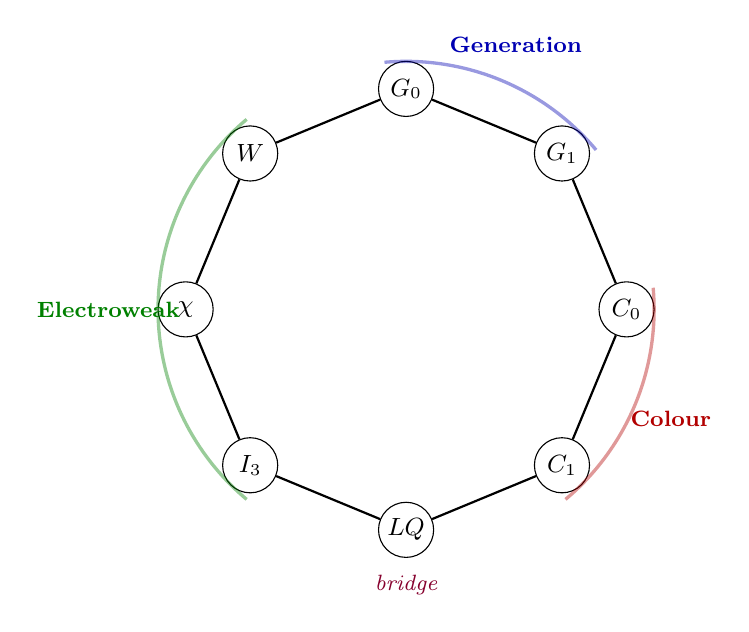
\begin{tikzpicture}[scale=1.4]
  % Bit positions (clockwise from top)
  \foreach \i/\label/\angle in {
    0/$G_0$/90, 1/$G_1$/45, 2/$C_0$/0, 3/$C_1$/-45,
    4/$LQ$/-90, 5/$I_3$/-135, 6/$\chi$/-180, 7/$W$/-225
  } {
    \node[circle, draw, fill=white, minimum size=0.7cm, inner sep=0pt] 
      (bit\i) at (\angle:2.0) {\small \label};
  }
  % Ring edges
  \foreach \i in {0,...,6} {
    \pgfmathtruncatemacro{\j}{\i+1}
    \draw[thick] (bit\i) -- (bit\j);
  }
  \draw[thick] (bit7) -- (bit0);
  % Sector labels
  \node[blue!70!black, font=\footnotesize\bfseries] at (67.5:2.6) {Generation};
  \node[red!70!black, font=\footnotesize\bfseries] at (-22.5:2.6) {Colour};
  \node[green!50!black, font=\footnotesize\bfseries] at (-180:2.7) {Electroweak};
  \node[purple!70!black, font=\footnotesize\itshape] at (-90:2.5) {bridge};
  % Sector arcs
  \draw[blue!70!black, very thick, opacity=0.4] (95:2.25) arc (95:40:2.25);
  \draw[red!70!black, very thick, opacity=0.4] (5:2.25) arc (5:-50:2.25);
  \draw[green!50!black, very thick, opacity=0.4] (-130:2.25) arc (-130:-230:2.25);
\end{tikzpicture}
\end{center}

On this ring, exactly four local constraints select the 45 valid states:

\begin{table}[H]
\centering
\caption{Local constraints on the ring.}
\label{tab:local_rules}
\begin{tabular}{c l l l}
\toprule
\textbf{Rule} & \textbf{Window} & \textbf{Forbidden} & \textbf{Meaning} \\
\midrule
R1 & $G_0, G_1$ & $(1,1)$ & No fourth generation \\
R2 & $\chi, W$ & $(0,1)$ or $(1,0)$ & Chirality = weak coupling \\
R3 & $C_1, LQ$ & $(1,0)$ & Leptons carry no colour \\
R4 & $LQ, I_3, \chi$ & $(0,0,1)$ & No right-handed neutrino \\
\bottomrule
\end{tabular}
\end{table}

All four rules involve \emph{adjacent} bits on the ring. There are no non-local constraints. This is a non-trivial result: there is no a priori reason why five independent physical laws should all reduce to local rules on a single topological structure.

\subsection{Antimatter as orientation}

The matter/antimatter distinction acquires a geometric interpretation: it is the \emph{orientation} of reading the ring. A matter particle is the ring read clockwise; its antiparticle is the same ring read anticlockwise. Charge conjugation $\mathcal{C}$ is the operation of reversing the reading direction. Combined with $\mathcal{P}$ (flip chirality bit $\chi$) and $\mathcal{T}$ (reverse the lattice update direction), this is consistent with the CPT theorem.

\subsection{Gauge group factorisation}

The ring topology mirrors the gauge group factorisation of the Standard Model. The colour sector ($C_0, C_1$) encodes $SU(3)_C$; the electroweak sector ($I_3, \chi, W$) encodes $SU(2)_L \times U(1)_Y$; the generation sector ($G_0, G_1$) encodes flavour. The bridge bit $LQ$ determines which sectors are active. This is the Standard Model's gauge structure written directly onto a topological object.


% ============================================================
% PART II: IT FROM COMPUTATION — THE DYNAMICS
% ============================================================

\part*{Part II: It from Computation}
\addcontentsline{toc}{part}{Part II: It from Computation}

% ============================================================
\section{Refining the CKM Hierarchy}
\label{sec:ckm_weighted}

\subsection{The discrepancy}

Section~\ref{sec:ckm_basic} showed that CKM elements correlate with Hamming distance between generation bit-pairs. However, the standard Hamming distance fails to distinguish $|V_{ub}|^2 \approx 1.3 \times 10^{-5}$ from $|V_{ts}|^2 \approx 1.6 \times 10^{-3}$, despite both corresponding to one-bit transitions ($00 \to 10$ and $01 \to 11$). This suggests the generation sector is \emph{hierarchical} rather than flat.

\subsection{Weighted Hamming distance}

We propose that the two generation bits carry different energy costs for flipping. Define the weighted distance:
\begin{equation}
\Delta(\mathbf{g}_i, \mathbf{g}_j) = w_1 |b_{1i} - b_{1j}| + w_2 |b_{2i} - b_{2j}|
\end{equation}
with mixing elements scaling as $|V_{ij}|^2 \propto \exp(-\alpha \, \Delta)$. If $b_1$ represents a ``coarse'' generational transition and $b_2$ a ``fine'' adjustment, then $w_1 \gg w_2$. Using the Wolfenstein parametrisation~\citep{Wolfenstein1983,PDG2024}, a fit identifies $w_1$ as the weight governing $1 \leftrightarrow 3$ transitions and $w_2$ as the weight governing $1 \leftrightarrow 2$ and $2 \leftrightarrow 3$ transitions, with $w_1/w_2 \approx 2$ in logarithmic suppression scale.

\subsection{Gray coding alternative}

An alternative uses a Gray code for the generation bits:
\begin{center}
\begin{tabular}{lccc}
\toprule
Generation & Standard & Gray code \\
\midrule
1 & 00 & 00 \\
2 & 01 & 01 \\
3 & 10 & 11 \\
\bottomrule
\end{tabular}
\end{center}
Under Gray coding, $1 \to 3$ requires two bit flips while $1 \to 2$ and $2 \to 3$ each require one, naturally reproducing $|V_{ub}| \ll |V_{us}|, |V_{cb}|$ without weights. A systematic $\chi^2$ fit to all nine elements would determine the optimal scheme.


% ============================================================
\section{Forces as Bit-Manipulation Operators}
\label{sec:forces}

\subsection{The principle}

Each known force couples to exactly one ring sector. We propose that gauge bosons are specific \emph{bit-manipulation operators} acting on the ring---``syndrome operators'' in coding-theoretic language.

\subsection{Gluons as colour permutation matrices}

The colour bits $(b_4, b_5)$ encode three non-trivial colour states for quarks: $(0,1)$, $(1,0)$, $(1,1)$. The eight gluons correspond to the generators of $SU(3)$ acting on this two-bit space: six directed colour transitions ($r \to g$, $g \to r$, etc.) plus two diagonal combinations---matching $3^2 - 1 = 8$ gluons exactly.

These operators preserve the constraint that $\mathbf{c} \neq (0,0)$, corresponding to the fact that gluons cannot turn a quark into a lepton. Colour confinement---the requirement that $b_4 \oplus b_5 = 0$ summed across constituents---is maintained because each gluon preserves XOR closure, just as syndrome operations preserve codeword parity in error-correcting codes.

\subsection{The $W$ boson as a conditional bit-flip}

The $W^{\pm}$ bosons change isospin ($b_6$) and only couple to left-handed particles. In ring language:
\begin{equation}
W^{\pm}: \quad \text{if } b_7 = 0 \text{ (left-handed)}, \quad \text{then flip } b_6 \text{ (isospin)}
\end{equation}
The condition $b_7 = 0$ encodes the parity-violating nature of the weak force as a gate condition on the operator. Rule R2 is thereby promoted from a static constraint to a \emph{dynamical selection rule}.

\subsection{The photon and the $Z$ boson}

The photon couples to electric charge $Q = b_3 - b_6$, a derived quantity spanning the bridge bit. This cross-sector nature---the photon depends on both the colour-sector boundary ($b_3$) and the electroweak sector ($b_6$)---may explain why electromagnetism is long-ranged: the photon operates on a derived combination rather than a native sector. The $Z$ boson reads the state of $b_6$ and $b_3$ without flipping them.

\subsection{Force hierarchy from ring structure}

The error-correcting code interpretation gives a natural force hierarchy. The strong force flips bits within the tightly-coupled colour sector (short range, high strength). The weak force flips bits conditionally within the electroweak sector (short range due to the chirality gate). Electromagnetism reads a derived cross-sector quantity (long range because the photon is massless). Gravity---as we show in Part III---is not a force on the ring at all but the geometry of the information space in which the ring operates.


% ============================================================
\section{Mass from Circulation Frequency}
\label{sec:mass}

\subsection{The mass gap}

The encoding explains particle identity, quantum numbers, and selection rules, but says nothing about why the top quark is $10^5$ times heavier than the electron. We offer two complementary proposals.

\subsection{Temporal resonance}

If a \circlette{} is a stable bit pattern on a surface updating at the Planck time ($t_P \approx 5.4 \times 10^{-44}$~s), mass could be proportional to the \emph{winding number} $\nu$---the number of complete information circuits per Planck time required to sustain the pattern:
\begin{equation}
m \propto \nu \cdot E_P / c^2
\end{equation}
Heavier particles are patterns that must ``refresh'' faster to persist. Quarks, which must satisfy both colour and electroweak constraints simultaneously, would generically be heavier than leptons, which satisfy only electroweak constraints.

\subsection{Bit-density}

Alternatively, mass scales with the number of surface bits required to maintain the pattern against vacuum fluctuations~\citep{Wheeler1990}. Higher-generation patterns require larger ``support regions'' and are therefore both heavier and less stable. The Higgs field, in this interpretation, is the lattice's resistance to supporting patterns---the background stiffness of the holographic surface.

\subsection{Predictions}

Both proposals predict: (1)~mass ratios between generations follow a roughly geometric progression; (2)~the neutrino mass hierarchy depends on whether the chirality constraint reduces or increases the winding number; (3)~the Higgs boson is a collective lattice excitation, not a \circlette{} pattern.


% ============================================================
\section{Grand Unification via the Bridge Bit}
\label{sec:unification}

The bridge bit $b_3$ separates quarks from leptons. Grand unified theories require their unification at high energies. We propose that $b_3$ is not a classical bit but a qubit:
\begin{equation}
|b_3\rangle = \alpha |0\rangle + \beta |1\rangle
\end{equation}
At high energies, $|\alpha| \approx |\beta|$ and the particle is simultaneously quark and lepton. As the universe cools, decoherence ``locks'' $b_3$ into $|0\rangle$ or $|1\rangle$, separating the sectors. Proton decay is the tunnelling amplitude for $b_3$ to return to superposition. The electroweak symmetry breaking is analogous: the chirality bit $b_7$ enters partial superposition at high energies, and its locking creates the $W/Z$ mass gap.


% ============================================================
\section{The Uncertainty Principle from Information Bounds}
\label{sec:uncertainty}

The Bekenstein bound~\citep{Bekenstein1981} limits the information $I$ of a system with energy $E$ in radius $R$: $I \leq 2\pi R E / \hbar c \ln 2$. If $N$ bits on a surface patch encode a particle's state, with $n_x$ bits for position and $N - n_x$ for momentum:
\begin{equation}
\Delta x \cdot \Delta p \sim \frac{LP}{2^N}
\end{equation}
This product is independent of how bits are allocated. With $L$ and $P$ at the Planck scale and $N$ at the Bekenstein limit, this recovers $\Delta x \cdot \Delta p \geq \hbar/2$. The uncertainty principle becomes a \emph{storage limitation}: conjugate variables draw on the same finite pool of bits.


% ============================================================
% PART III: IT FROM GEOMETRY — GRAVITY AND SPACETIME
% ============================================================

\part*{Part III: It from Geometry}
\addcontentsline{toc}{part}{Part III: It from Geometry}

% ============================================================
\section{The Lattice Substrate}
\label{sec:spacetime}

The holographic principle~\citep{Bekenstein1973,Susskind1995} bounds the information in a volume by its boundary area, at one bit per Planck area. We take this literally: the universe \emph{is} a two-dimensional lattice of bits, updating synchronously at the Planck time, governed by a deterministic local rule~\citep{tHooft2016,Zuse1969}.

The 3+1 dimensions we experience are the \emph{error-corrected logical content} of this 2D lattice---analogous to how a quantum error-correcting code encodes $k$ logical qubits in $n$ physical qubits. Time is the update tick. The arrow of time is the direction of computation. A \circlette{} is a stable, self-propagating pattern on the lattice---a ``glider'' in cellular automaton terminology~\citep{Wolfram2002}.


% ============================================================
\section{Gravity as Lattice Tension}
\label{sec:gravity}

Gravity is not mediated by a boson. It is the \emph{curvature of the lattice caused by information density}. Where \circlette{} patterns cluster, the lattice allocates more bits per unit area, distorting local connectivity. Nearby patterns converge not because a graviton pulls them but because the distorted geometry makes convergent paths shorter---exactly as in general relativity~\citep{Verlinde2011,Jacobson1995}.

Gravitational time dilation is computational congestion: regions of high pattern density have less spare capacity. The speed of light $c$ is the lattice's maximum propagation speed. Lorentz invariance is exact at macroscopic scales but may show violations at the Planck scale---a testable prediction.


% ============================================================
\section{Information Geometry: The Bridge to General Relativity}
\label{sec:info_geometry}

\subsection{Overview}

The previous section described gravity as ``lattice tension.'' Here we formalise this as a quantitative bridge from the discrete lattice to the continuous Riemannian geometry of general relativity, using the tools of information geometry~\citep{Amari2016}.

The key idea: the lattice at each site has a statistical state---a probability distribution over local bit configurations. The Fisher information metric on this statistical manifold is a natural Riemannian metric. Our claim is that this Fisher metric, in the continuum limit, \emph{is} the spacetime metric $g_{\mu\nu}$.

\subsection{The update rule as a Markov chain}

Let $U$ denote the global update rule. Restricting to a local patch of $M$ sites at position $\boldsymbol{\theta}$, the deterministic dynamics induce a stochastic process (the boundary conditions are unknown to the local observer):
\begin{equation}
p_{t+1}(\mathbf{b}\,|\,\boldsymbol{\theta}) = \sum_{\mathbf{b}'} T(\mathbf{b}\,|\,\mathbf{b}', \boldsymbol{\theta}) \, p_t(\mathbf{b}'\,|\,\boldsymbol{\theta})
\end{equation}
For a stable \circlette{} pattern, this converges to a steady state $p^*(\mathbf{b}\,|\,\boldsymbol{\theta})$ satisfying $p^* = Tp^*$.

The mutual information between a cell and its neighbourhood,
\begin{equation}
I(b_i ; \mathbf{b}_{\mathcal{N}(i)}) = H(b_i) + H(\mathbf{b}_{\mathcal{N}(i)}) - H(b_i, \mathbf{b}_{\mathcal{N}(i)})
\end{equation}
is high inside a \circlette{} (bits are predictable from context) and low in vacuum (maximally entropic). The spatial gradient of this mutual information landscape generates Fisher curvature.

\subsection{The Fisher metric and its identification with $g_{\mu\nu}$}

The Fisher information matrix at $\boldsymbol{\theta}$ is:
\begin{equation}
\mathcal{F}_{ij}(\boldsymbol{\theta}) = \sum_{\mathbf{b}} p^*(\mathbf{b}\,|\,\boldsymbol{\theta}) \, \frac{\partial \ln p^*(\mathbf{b}\,|\,\boldsymbol{\theta})}{\partial \theta^i} \, \frac{\partial \ln p^*(\mathbf{b}\,|\,\boldsymbol{\theta})}{\partial \theta^j}
\end{equation}
We propose:
\begin{equation}
\label{eq:metric_id}
\boxed{g_{ij}(\boldsymbol{\theta}) = \frac{\ell_P^2}{\kappa} \, \mathcal{F}_{ij}(\boldsymbol{\theta})}
\end{equation}

This identification has four consequences. \emph{Matter determines geometry}: more \circlettes{} produce sharper distributions and larger Fisher curvature. \emph{Vacuum is flat}: uniform $p^*$ gives vanishing $\mathcal{F}_{ij}$, yielding Minkowski space. \emph{Geodesics are natural}: Fisher geodesics are paths of maximal statistical distinguishability, i.e.\ paths of least information loss---which are the geodesics of $g_{ij}$ in the continuum. \emph{Curvature is computable}: given the update rule and \circlette{} encoding, $\mathcal{F}_{ij}$ is derivable rather than postulated.

\begin{figure}[H]
\centering
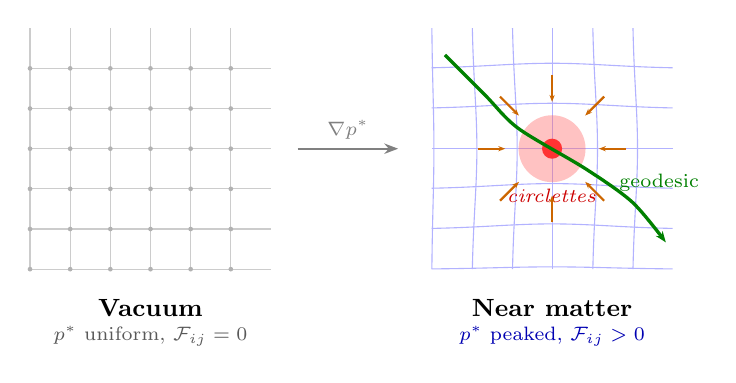
\begin{tikzpicture}[scale=0.85]
  % ---- LEFT: Vacuum (flat) ----
  % Grid lines - uniform spacing
  \foreach \x in {0,0.6,...,3.6} {
    \draw[gray!40, thin] (\x,0) -- (\x,3.6);
  }
  \foreach \y in {0,0.6,...,3.6} {
    \draw[gray!40, thin] (0,\y) -- (3.6,\y);
  }
  % Dots at intersections
  \foreach \x in {0,0.6,...,3.6} {
    \foreach \y in {0,0.6,...,3.6} {
      \fill[black!30] (\x,\y) circle (1pt);
    }
  }
  \node[below, font=\small\bfseries] at (1.8,-0.3) {Vacuum};
  \node[below, font=\scriptsize, text=gray!70!black] at (1.8,-0.7) {$p^*$ uniform, $\mathcal{F}_{ij} = 0$};

  % ---- RIGHT: Near circlette cluster (curved) ----
  \begin{scope}[xshift=6cm]
    % Centre of mass
    \coordinate (C) at (1.8,1.8);
    
    % Curved grid lines - converging toward centre
    % Vertical lines, pulled inward near centre
    \foreach \rawx in {0,0.6,...,3.6} {
      \draw[blue!30, thin] plot[smooth, samples=20, domain=0:3.6] 
        ({\rawx + 0.3*exp(-( (\rawx-1.8)*(\rawx-1.8) + (\x-1.8)*(\x-1.8) )/1.5) * (\rawx < 1.8 ? 1 : -1) * (1.8-\rawx)/1.8}, {\x});
    }
    % Horizontal lines, pulled inward near centre
    \foreach \rawy in {0,0.6,...,3.6} {
      \draw[blue!30, thin] plot[smooth, samples=20, domain=0:3.6] 
        ({\x}, {\rawy + 0.3*exp(-( (\x-1.8)*(\x-1.8) + (\rawy-1.8)*(\rawy-1.8) )/1.5) * (\rawy < 1.8 ? 1 : -1) * (1.8-\rawy)/1.8});
    }
    
    % Circlette cluster at centre
    \fill[red!60, opacity=0.4] (C) circle (0.5);
    \fill[red!80] (C) circle (0.15);
    \node[font=\scriptsize, red!80!black] at (1.8,1.1) {\circlettes{}};
    
    % Gradient arrows showing ∇p*
    \foreach \angle in {0,45,...,315} {
      \draw[-{Stealth[length=2.5pt]}, orange!80!black, thick] 
        ({1.8 + 1.1*cos(\angle)},{1.8 + 1.1*sin(\angle)}) -- 
        ({1.8 + 0.7*cos(\angle)},{1.8 + 0.7*sin(\angle)});
    }
    
    % Geodesic (curved path)
    \draw[green!50!black, very thick, -{Stealth[length=4pt]}] 
      plot[smooth] coordinates {(0.2,3.2) (0.8,2.6) (1.3,2.1) (2.3,1.5) (3.0,1.0) (3.5,0.4)};
    \node[font=\scriptsize, green!50!black] at (3.4,1.3) {geodesic};
    
    \node[below, font=\small\bfseries] at (1.8,-0.3) {Near matter};
    \node[below, font=\scriptsize, text=blue!70!black] at (1.8,-0.7) {$p^*$ peaked, $\mathcal{F}_{ij} > 0$};
  \end{scope}

  % Arrow between panels
  \draw[-{Stealth[length=5pt]}, thick, gray] (4.0,1.8) -- (5.5,1.8);
  \node[above, font=\scriptsize, gray] at (4.75,1.8) {$\nabla p^*$};
\end{tikzpicture}
\caption{Visualising the Fisher metric. \textbf{Left}: Vacuum region---uniform bit-distribution $p^*$, flat Fisher metric, parallel lattice lines. \textbf{Right}: Near a \circlette{} cluster---sharply peaked $p^*$, non-zero $\mathcal{F}_{ij}$, converging lattice lines. Orange arrows show the bit-density gradient $\nabla p^*$ that generates Fisher curvature. The green curve is a Fisher geodesic (free-fall trajectory), deflected by the curvature exactly as in general relativity.}
\label{fig:fisher}
\end{figure}

\begin{figure}[H]
\centering
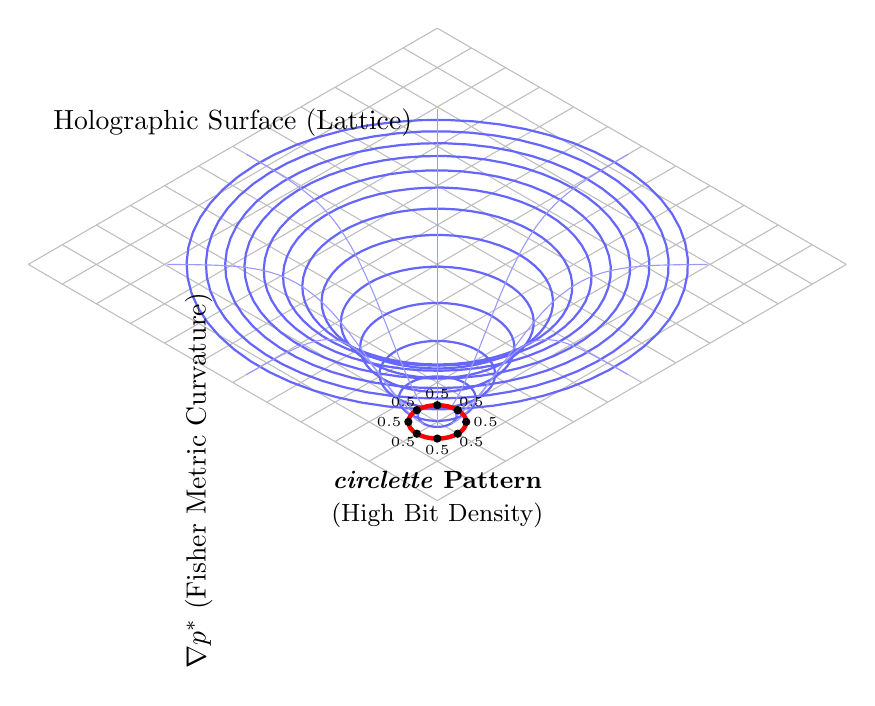
\begin{tikzpicture}[x={(0.866cm,0.5cm)}, y={(-0.866cm,0.5cm)}, z={(0cm,1cm)}]
  \pgfmathsetseed{42}
  % Draw the "Spacetime" Grid (Fisher Manifold)
  \begin{scope}[canvas is xy plane at z=0]
    \draw[lightgray, step=0.5] (-3,-3) grid (3,3);
  \end{scope}

  % Draw the Curvature (The Information Well)
  \foreach \r in {0,0.2,...,2.6} {
    \draw[blue!60, thick] plot[domain=0:360, samples=60]
      ({\r*cos(\x)}, {\r*sin(\x)}, {-2*exp(-\r*\r)});
  }

  % Draw Radial Geodesics (Lines of Information Flow)
  \foreach \ang in {0,45,...,315} {
    \draw[blue!40] plot[domain=0.2:2.8, samples=30]
      ({\x*cos(\ang)}, {\x*sin(\ang)}, {-2*exp(-\x*\x)});
  }

  % The "Circlette" at the bottom of the well
  \begin{scope}[shift={(0,0,-2)}]
    \draw[red, ultra thick] (0,0) circle (0.3);
    \foreach \a in {0,45,...,315} {
      \fill[black] (\a:0.3) circle (1.5pt);
      \pgfmathparse{int(mod(\a/45,2))}%
      \node at (\a:0.5) {\tiny \pgfmathresult};
    }
  \end{scope}

  % Labels
  \node[anchor=south] at (0,3,0) {Holographic Surface (Lattice)};
  \node[anchor=north, text width=3cm, align=center] at (0,0,-2.5)
    {\small \textbf{\circlette{} Pattern} \\ (High Bit Density)};
  \node[rotate=90] at (-3.5,0,-1) {$\nabla p^*$ (Fisher Metric Curvature)};
\end{tikzpicture}
\caption{The Fisher information well. The flat grid at the top represents the holographic lattice in vacuum (uniform $p^*$, flat $\mathcal{F}_{ij}$). The blue funnel shows how the Fisher manifold curves downward where a \circlette{} pattern (red ring at the bottom) creates a region of high bit-density. Radial blue lines are geodesics of the Fisher metric---paths of least information loss. A test pattern following these geodesics falls toward the \circlette{}, exactly as a test mass falls in a Schwarzschild gravitational well. The depth of the well is proportional to $\mathcal{F}^{\text{local}}$, which is proportional to the pattern's mass (winding number $\nu$).}
\label{fig:well}
\end{figure}

\subsection{The Information Action Principle}
\label{sec:info_action}

The identification of geodesics with paths of least information loss has a deeper consequence when combined with the path integral (Section~\ref{sec:quantum}). It yields a unified variational principle that connects Feynman's sum over histories to gravitational dynamics, and produces a conservation law.

\subsubsection{The information action}

Define the \emph{information action} along a path $\gamma$ through the lattice as the total Fisher length of the path:
\begin{equation}
\label{eq:info_action}
S_I[\gamma] = \int_\gamma \sqrt{\mathcal{F}_{ij}(\boldsymbol{\theta}) \, d\theta^i \, d\theta^j}
\end{equation}
This measures the cumulative statistical distinguishability traversed by the \circlette{} pattern as it moves from point $A$ to point $B$ on the lattice. It is the information-geometric analogue of the classical action $S = \int L \, dt$.

\emph{Continuum limit.} Equation~\eqref{eq:info_action} uses an integral, but the lattice is discrete. The justification is that the lattice density is $1/\ell_P^2 \approx 3.8 \times 10^{69}$~sites/m$^2$. Any macroscopic path of length $L$ traverses $\sim L/\ell_P$ lattice steps. The discrete Fisher sum $S_I^{\text{disc}} = \sum_{k=1}^{N} \sqrt{\mathcal{F}_{ij} \, \Delta\theta^i_k \, \Delta\theta^j_k}$ converges to the Riemannian integral~\eqref{eq:info_action} by the standard Riemann sum argument, with corrections at order $\ell_P/L$. These corrections are unobservable for any path longer than the Planck length---but they become significant at Planck-scale energies, where the discrete structure of the sum produces measurable effects (Section~\ref{sec:decoherence}).

The Fisher geodesic---the classical trajectory---minimises $S_I$. It is the path along which the pattern's statistical identity changes \emph{least}: the pattern arrives at $B$ maximally resembling what it was at $A$. This is free fall. A pattern in free fall preserves its bit-structure with minimal distortion.

\subsubsection{The path integral over information paths}

The Feynman propagator for a \circlette{} moving from $A$ to $B$ is:
\begin{equation}
\label{eq:info_propagator}
K(A \to B) = \sum_{\gamma: A \to B} \exp\!\left(\frac{i \, S_I[\gamma]}{\hbar_I}\right)
\end{equation}
where $\hbar_I = \ell_P^2 / \kappa$ is the information-geometric analogue of Planck's constant, set by the same coupling that relates $\mathcal{F}_{ij}$ to $g_{ij}$ in equation~\eqref{eq:metric_id}. The sum is over \emph{all} lattice paths from $A$ to $B$, not just the geodesic.

In the classical limit ($S_I \gg \hbar_I$), stationary phase selects the Fisher geodesic: the classical trajectory dominates the sum. Off-geodesic paths contribute with rapidly oscillating phases that cancel. But in the quantum regime, paths that deviate from the geodesic contribute finite amplitudes---these are the quantum corrections to gravitational motion.

This has a precise physical meaning. Each off-geodesic path corresponds to a trajectory along which the \circlette{} pattern \emph{loses more information}---its statistical identity is degraded by the detour through regions of different $p^*$. The pattern arrives at $B$ less ``like itself'' than it would via the geodesic. The path integral sums these degraded contributions with appropriate phases, producing interference effects that are the gravitational analogues of quantum diffraction.

\emph{The origin of $i$.} In a deterministic cellular automaton~\citep{tHooft2016}, the imaginary unit $i$ in the propagator~\eqref{eq:info_propagator} is not a property of the lattice itself (which is real-valued and deterministic). It arises from the coarse-graining map. The lattice's microstate space has dimension $2^N$; the macrostate space accessible to observation is vastly smaller. The projection from microstates to macrostates naturally induces a complex Hilbert space structure, with $e^{iS_I/\hbar_I}$ encoding the relative phase between microstate paths that map to the same macroscopic trajectory~\citep{tHooft2016}. In the lattice framework, there is an additional geometric interpretation: for a 2D holographic surface, the phase $i$ may correspond to a $\pi/2$ rotation in the lattice plane, so that the path integral phase is literally the geometric (Berry) phase accumulated by the pattern as it circulates on the surface.

\subsubsection{Lattice-induced decoherence}
\label{sec:decoherence}

The discrete structure of the lattice introduces a prediction absent from continuum quantum mechanics. On the lattice, the information action is quantised: each lattice step contributes a finite increment $\delta S_I \sim \sqrt{\mathcal{F}_{ij} \, \ell_P^2}$ to the total action. For paths where the total $S_I$ is large---either because the path is long or because it traverses regions of steep Fisher curvature---the phase $e^{iS_I/\hbar_I}$ oscillates rapidly from step to step.

For a \circlette{} with winding number $\nu$ (Section~\ref{sec:mass}), the information action per lattice step scales as $\delta S_I \propto \nu$: heavier patterns undergo more statistical identity change per step, because their bit-structure is more complex and therefore more sensitive to Fisher curvature gradients. This means:

\begin{enumerate}[nosep]
  \item \textbf{Mass-dependent decoherence}: Heavier particles lose coherence faster than lighter ones when traversing regions of high curvature. The decoherence rate scales as $\Gamma_{\text{dec}} \propto \nu^2 \, \mathcal{F}^{\text{local}}$---the product of the pattern's complexity squared and the local Fisher curvature.
  
  \item \textbf{High-energy identity loss}: At energies approaching the Planck scale, paths probe the lattice's discrete structure. The $\ell_P$ corrections to the continuum limit (noted above) become significant. Patterns on such paths undergo rapid statistical identity change---their bit-configurations ``blur'' across multiple \circlette{} types---explaining why we do not observe stable massive particles in the highest-energy tails of collision experiments: their information action per step exceeds the coherence threshold.
  
  \item \textbf{Gravitational decoherence}: Near massive objects (where $\mathcal{F}_{ij}$ is large), all patterns experience enhanced decoherence. This is a specific, testable prediction: quantum interference experiments in different gravitational potentials should show gravity-dependent decoherence rates beyond the standard time-dilation effect. The additional lattice contribution scales as $\ell_P^2 \, \nabla^2 \mathcal{F}$ and is extremely small but non-zero.
\end{enumerate}

This lattice-induced decoherence is distinct from environmental decoherence (which involves interaction with other systems) and from gravitational decoherence proposals based on semiclassical gravity (which treat the metric as classical). Here, the decoherence arises from the discreteness of the information substrate itself---it is an intrinsic property of the lattice, not an environmental effect.

\subsubsection{Conservation of information current and the emergence of momentum}

The variational principle $\delta S_I = 0$ applied to the information action yields the geodesic equation on the Fisher manifold:
\begin{equation}
\label{eq:fisher_geodesic}
\frac{d^2 \theta^k}{ds^2} + \Gamma^k_{\;ij} \frac{d\theta^i}{ds} \frac{d\theta^j}{ds} = 0
\end{equation}
where $\Gamma^k_{\;ij}$ are the Christoffel symbols of $\mathcal{F}_{ij}$ and $s$ is the Fisher arc-length parameter. Since $g_{ij} \propto \mathcal{F}_{ij}$, these are \emph{exactly} the Christoffel symbols of the spacetime metric, and equation~\eqref{eq:fisher_geodesic} is \emph{exactly} the geodesic equation of general relativity.

Associated with this variational symmetry is a conserved quantity. Define the \emph{information current} $J^\mu$ along the trajectory:
\begin{equation}
\label{eq:info_current}
J^\mu = p^*(\mathbf{b}\,|\,\boldsymbol{\theta}) \, \frac{d\theta^\mu}{ds}
\end{equation}
This is the rate at which the pattern's statistical weight is transported through the Fisher manifold. By Noether's theorem applied to the translation invariance of $S_I$, the information current satisfies a continuity equation:
\begin{equation}
\label{eq:info_conservation}
\nabla_\mu J^\mu = 0
\end{equation}
This is the \emph{conservation of information current}: the total statistical weight carried by a freely-falling \circlette{} pattern is conserved along its worldline. Information is neither created nor destroyed in free fall.

\emph{Conservation of Bit-Identity.} We may state equation~\eqref{eq:info_conservation} more precisely as a \emph{Conservation of Bit-Identity} law: a \circlette{} pattern propagating on a Fisher geodesic preserves its integrated statistical distinguishability---the quantity that makes it ``this particle and not another''---at every point along its worldline. This is the information-geometric origin of particle identity persistence.

\emph{The emergence of momentum and energy.} The standard conservation laws of physics follow from the symmetries of the update rule $U$ via Noether's theorem applied to $S_I$:

\begin{enumerate}[nosep]
  \item If $U$ is \emph{spatially translation-invariant} on the lattice (the same rule at every site), then $S_I$ is invariant under spatial translations $\theta^i \to \theta^i + a^i$. Noether's theorem gives a conserved spatial current $\pi_i = \mathcal{F}_{ij} \, d\theta^j/ds$. This is \emph{momentum}. Momentum is not a primitive quantity; it is the Noether charge of lattice translation symmetry, mediated by the Fisher metric.
  
  \item If $U$ is \emph{temporally translation-invariant} (the same rule at every tick), then $S_I$ is invariant under time translations. The conserved charge is $E = \mathcal{F}_{0j} \, d\theta^j/ds$. This is \emph{energy}. Energy conservation is the statement that the update rule does not change over time.
  
  \item If $U$ is \emph{rotationally symmetric} on the lattice (the rule is isotropic), the conserved charge is \emph{angular momentum} $L_k = \epsilon_{kij} \, \theta^i \, \mathcal{F}^{jl} \, d\theta_l/ds$.
\end{enumerate}

All three conservation laws emerge from the same structure: the symmetries of the update rule, transmitted through the Fisher metric via the information action. No additional postulates are required. The update rule's symmetries \emph{are} the conservation laws, expressed in information-geometric language.

\subsubsection{Physical interpretation}

The conservation law~\eqref{eq:info_conservation} is the information-geometric counterpart of the conservation of the stress-energy tensor $\nabla_\mu T^{\mu\nu} = 0$ in general relativity. It states that a pattern propagating along a Fisher geodesic maintains its total ``information charge''---the integrated statistical distinguishability that defines its identity as a particle.

When a force acts (a gauge boson operator flips bits on the ring, as in Section~\ref{sec:forces}), the pattern is pushed off the Fisher geodesic. The information action increases. The pattern's statistical identity is partially degraded. The force is, in information-geometric terms, a \emph{source of distinguishability change}---it costs information to deviate from free fall, just as it costs energy in the standard formulation.

This unifies three apparently separate structures:
\begin{enumerate}[nosep]
  \item \textbf{Classical gravity}: The geodesic equation~\eqref{eq:fisher_geodesic} as the path of least information loss.
  \item \textbf{Quantum mechanics}: The path integral~\eqref{eq:info_propagator} as the sum over all information paths, with the geodesic dominating classically.
  \item \textbf{Conservation laws}: The continuity equation~\eqref{eq:info_conservation} as Noether's consequence of translational symmetry on the Fisher manifold.
\end{enumerate}
In the standard formulation, these are three different mathematical frameworks (Riemannian geometry, functional integration, Noether theory) applied to three different domains (gravity, quantum mechanics, symmetries). In the information-geometric framework, they are three aspects of a single structure: the Fisher metric on the lattice's statistical manifold.

\subsection{From Fisher curvature to Einstein's equations}

Following Jacobson~\citep{Jacobson1995}, translated into lattice language:

\begin{enumerate}[nosep]
  \item \textbf{Local Rindler horizons} are well-defined combinatorial objects on the lattice, determined by the update rule's propagation speed.
  \item \textbf{The Clausius relation} $\delta Q = T\,dS$ holds: $\delta Q$ is pattern density crossing the horizon, $T$ is the Unruh temperature (proportional to local acceleration), $S$ is the Shannon entropy of the horizon bits.
  \item \textbf{Entropy is proportional to area}---the Bekenstein--Hawking relation---which is the \emph{starting postulate} of the entire \circlette{} framework.
  \item \textbf{Einstein's equations follow} uniquely from (1)--(3) applied to all local horizons~\citep{Jacobson1995}.
\end{enumerate}

The stress-energy tensor is identified with the gradient of bit-density:
\begin{equation}
T_{ij} \propto \nabla_i p^* \, \nabla_j p^*
\end{equation}
connecting $T_{ij}$ directly to $\mathcal{F}_{ij}$, since the Fisher metric is built from derivatives of $\ln p^*$.

\subsection{Schwarzschild limit}

For a single isolated \circlette{} with Gaussian profile $p^*(\mathbf{b}_{\text{pattern}}\,|\,\boldsymbol{\theta}) \propto \exp(-|\boldsymbol{\theta}|^2/2\sigma^2)$, the Fisher metric acquires $\mathcal{F}_{rr} \propto r^2/\sigma^4 \exp(-r^2/\sigma^2)$, which decays as $1/r^2$ in the far field---reproducing the Newtonian potential and the weak-field Schwarzschild metric $g_{tt} \approx -(1 - 2GM/rc^2)$ when $\sigma$ and the pattern amplitude are matched to the particle's mass.

\subsection{The cosmological constant as information floor}

Even without \circlette{} patterns, the update rule runs. If the vacuum state exhibits residual dynamics, the vacuum distribution $p^*_{\text{vac}}$ is not exactly uniform, producing a baseline Fisher curvature:
\begin{equation}
\Lambda = \frac{1}{\ell_P^2} \, \mathcal{F}^{\text{vac}}
\end{equation}
This is the \emph{information floor}---the minimum bit density for causal connectivity (the percolation threshold). The cosmological constant problem is reframed: QFT counts total vacuum energy; the lattice counts connectivity cost. These are different quantities, explaining the $\sim 10^{120}$ discrepancy without fine-tuning.

For a specific update rule, $\Lambda$ becomes calculable: determine the vacuum steady state, compute its Fisher information, take the trace. The cosmological constant becomes a derived quantity rather than a free parameter.

\subsection{The Computational Equivalence Principle}

\textbf{Inertial mass} is the cost of re-allocating lattice bits to change a pattern's trajectory. \textbf{Gravitational mass} is the pattern's contribution to Fisher curvature via locked bits. Both measure the same quantity: the pattern's \emph{lattice bandwidth cost}---the number of bits required to encode and maintain the pattern per unit time. A pattern that costs more bits is simultaneously harder to redirect (higher inertial mass) and creates more Fisher curvature (higher gravitational mass). The equivalence of inertial and gravitational mass---experimentally verified to $|m_i - m_g|/m < 10^{-15}$---becomes a mathematical identity rather than a postulate.

\subsection{The computational complexity bound}
\label{sec:complexity}

The lattice has finite computational bandwidth: one bit-operation per Planck time ($t_P$) per Planck area ($\ell_P^2$). This imposes an absolute upper limit on the complexity of any \circlette{} pattern that can be sustained in a given region.

\subsubsection{The Planck mass as a saturation limit}

A \circlette{} pattern with winding number $\nu$ (Section~\ref{sec:mass}) requires $\sim \nu$ bit-operations per tick to refresh. The lattice region supporting the pattern has area $A \sim \sigma^2$ (where $\sigma$ is the pattern's support radius). The local computational throughput is $A / \ell_P^2$ operations per tick. The pattern is sustainable only if:
\begin{equation}
\nu \leq \frac{\sigma^2}{\ell_P^2}
\end{equation}
When this bound is saturated---when the pattern demands every available bit-operation in its support region---the pattern's mass reaches the Planck mass $m_P = \sqrt{\hbar c / G} \approx 2.2 \times 10^{-8}$~kg. Beyond this, the lattice cannot sustain the pattern: it collapses into a configuration where the computational resources are entirely consumed by maintaining the boundary (a horizon). This is a black hole.

\subsubsection{Connection to ``Complexity Equals Action''}

Susskind and collaborators have conjectured that the computational complexity of a quantum state dual to a black hole interior grows linearly with time, at a rate bounded by the action~\citep{Susskind2016}. In our framework, this conjecture has a natural interpretation: the ``action'' in the Complexity Equals Action conjecture \emph{is} the information action $S_I$, and the ``complexity'' is the total number of lattice bit-operations required to evolve the state. The linear growth of complexity corresponds to the steady accumulation of Fisher arc-length as the lattice updates---each tick adds $\delta S_I$ to the total.

The black hole interior is a region where the lattice's computational capacity is fully committed to maintaining the horizon pattern. The ``complexity growth'' inside the horizon is the lattice's ongoing effort to process the information trapped behind it. The firewall paradox---whether an observer falling through a horizon encounters a singular surface---is reframed as a question about computational phase transitions: does the lattice's update rule admit a smooth transition from sub-saturated to saturated computation, or is there a sharp boundary? If the update rule is continuous (no phase transition), the horizon is smooth; if discontinuous, there is a firewall.

This connects the microscopic information structure of the \circlette{} framework to some of the deepest open questions in quantum gravity.


% ============================================================
\section{The Path Integral from Lattice Reversibility}
\label{sec:quantum}

If the lattice rule is reversible~\citep{Landauer1961}, the lattice is a bijection on its state space. Each macroscopic state maps to many microstates. The transition amplitude between macrostates involves summing over all microstate paths consistent with boundary conditions---the Feynman path integral~\citep{Feynman1982}.

The path integral need not be postulated; it \emph{follows} from deterministic, reversible lattice dynamics viewed through coarse-graining. The phases $e^{iS/\hbar}$ correspond to relative densities of microstate paths. Superposition is the natural state of underdetermined bits. Measurement is constraint propagation from the apparatus's own \circlettes{}. Entanglement is a pre-existing shared constraint resolved simultaneously at both endpoints---no signal, no mystery.

The connection to information geometry (Section~\ref{sec:info_action}) completes the picture. The classical action $S$ in the path integral is identified with the information action $S_I$---the integrated Fisher distance along the path. The classical trajectory (Fisher geodesic) dominates in the stationary-phase limit, reproducing both Newton's laws and the geodesic equation. Off-geodesic paths, which degrade the pattern's statistical identity, contribute quantum corrections. The conservation of information current (equation~\ref{eq:info_conservation}) provides the Noether charge associated with this variational structure.

Thus the three pillars of fundamental physics---the geodesic equation (gravity), the path integral (quantum mechanics), and Noether's theorem (conservation laws)---emerge as three aspects of a single information-geometric variational principle on the lattice.


% ============================================================
% PART IV: THE RULE
% ============================================================

\part*{Part IV: The Unique Weak Rule}
\addcontentsline{toc}{part}{Part IV: The Unique Weak Rule}

% ============================================================
\section{The Selection Principle}
\label{sec:update}

The information action principle (Section~\ref{sec:info_action}) does not merely constrain the update rule---it \emph{selects} one. We searched all invertible matrices over $\mathbb{F}_2$ that act at sector boundaries of the 8-bit ring, applying three constraints simultaneously:

\begin{enumerate}[nosep]
  \item \textbf{Invertibility}: The rule must be reversible (required by information conservation and for the path integral to emerge).
  \item \textbf{Spectrum preservation}: The rule must map the set of 45 valid states into pure-valid cycles (no valid state may evolve into an invalid state).
  \item \textbf{Minimum information action}: Among all rules satisfying (1) and (2), the rule must minimise the average bit-flip cost per state per tick.
\end{enumerate}

\textbf{Exactly one non-trivial rule survives all three filters.}


% ============================================================
\section{The Rule: $I_3(t+1) = I_3(t) \oplus LQ(t)$}
\label{sec:the_rule}

The unique rule is:
\begin{equation}
\label{eq:the_rule}
\boxed{b_5(t+1) = b_5(t) \oplus b_4(t)}
\end{equation}
with all other bits unchanged. In physical language: the isospin bit $I_3$ gets XORed with the bridge bit $LQ$ at every tick. The update matrix is:
\begin{equation}
M = I_8 + \mathbf{e}_5 \mathbf{e}_4^T \quad \text{over } \mathbb{F}_2
\end{equation}
where $\mathbf{e}_i$ is the $i$-th standard basis vector. This is the identity matrix with a single additional 1 at position $(5,4)$---the entry coupling the bridge bit to isospin.

\subsection{Action on the particle spectrum}

For \textbf{leptons} ($LQ = 0$): the XOR adds zero. $I_3$ is unchanged. All 9 lepton states---$\nu_e$, $e^-$, $\nu_\mu$, $\mu^-$, $\nu_\tau$, $\tau^-$ in both chiralities---are \emph{fixed points} of the rule.

For \textbf{quarks} ($LQ = 1$): the XOR flips $I_3$ at every tick. All 36 quark states oscillate in pairs of period 2:
\begin{equation}
u \leftrightarrow d, \quad c \leftrightarrow s, \quad t \leftrightarrow b
\end{equation}
independently for each colour ($r, g, b$) and chirality ($L, R$). The oscillating pairs are \emph{exactly} the weak isospin doublets of the Standard Model.

\subsection{Properties}

\emph{Order}: $M^2 = I$ over $\mathbb{F}_2$. The rule is an involution---a $\mathbb{Z}_2$ symmetry.

\emph{Bit-flip cost}: The average is $36/45 = 0.80$ bits per state per tick (36 quarks flip one bit each; 9 leptons flip none). This is the minimum possible for any non-trivial rule preserving all 45 states.

\emph{Why XOR}: XOR is the unique logic operation that is simultaneously linear, involutory ($a \oplus a = 0$), and bijective in $\mathbb{F}_2$. It is the simplest possible ``change that is its own undoing''---ensuring time-symmetry at the Planck scale while producing non-trivial dynamics at the macroscopic scale.


% ============================================================
\section{Physical Consequences}
\label{sec:consequences}

\subsection{The weak force as minimum information action}

The rule embeds the weak interaction directly. The $W$ boson mediates $u \leftrightarrow d$ transitions; the rule does exactly this, as the minimum-cost information exchange at the bridge-isospin boundary. The weak force is not merely compatible with the \circlette{} structure---it is \emph{required} by the information action principle. It is the cheapest possible non-trivial dynamics on the ring.

\subsection{Parity violation as a hardware constraint}

In the Standard Model, the $V-A$ structure of the weak interaction (coupling only to left-handed particles) is postulated. In our framework, Rule R2 ($\chi = W$: chirality equals weak participation) is a topological constraint on the ring. The weak rule~\eqref{eq:the_rule} physically cannot execute on right-handed neutrinos because Rule R4 blocks the state $(LQ=0, I_3=0, \chi=1)$. Parity violation is not a dynamical symmetry breaking---it is a \emph{hardware constraint} of the ring architecture. The weak force has no ``wire'' connected to right-handed neutrino states.

\subsection{CKM mixing from rule locality}

The rule operates exclusively at the $LQ$-$I_3$ boundary. The generation bits ($G_0, G_1$) are untouched. Generation-changing transitions---the off-diagonal CKM elements---can therefore only arise as secondary effects: perturbative corrections from the 2D lattice environment, or higher-order compositions with other boundary couplings. This naturally produces exponential suppression with Hamming distance (Section~\ref{sec:ckm_basic}): same-generation transitions are the fundamental rule; cross-generation transitions require ``tunnelling'' through the generation sector. The CKM hierarchy is not fitted but \emph{derived from the locality of the rule}.

Flavour-changing neutral currents (FCNC) are suppressed for the same reason: the rule couples $I_3$ to $LQ$, not to $G_0$ or $G_1$. Neutral currents that change flavour would require a rule acting at the generation-colour boundary---a different, higher-cost coupling that the information action principle selects against.

\subsection{Neutrino oscillation from vacuum interaction}

For leptons, the rule is the identity. Any oscillation in the lepton sector cannot come from the primary weak rule. It must arise from a separate, much weaker mechanism: interaction with the vacuum lattice's residual Fisher curvature $\mathcal{F}^{\text{vac}}$.

This yields a prediction: neutrino mass should scale with the vacuum Fisher information (the cosmological constant $\Lambda$), not with the weak coupling $G_F$. The observed smallness of neutrino masses ($m_\nu \sim 10^{-2}$~eV vs $m_W \sim 80$~GeV) would then reflect the ratio $\Lambda / G_F$---relating the two most puzzling scales in physics through a single information-geometric mechanism.

\subsection{The $W$ boson mass from bit-flip cost}

Quarks have an internal tick rate of 2 (period of the isospin oscillation). This constant bit-flipping represents a sustained information current. The energy required to initiate or halt this oscillation at the bridge is the $W$ boson mass. Specifically:
\begin{equation}
m_W \sim \frac{\delta S_I}{\ell_P \, c}
\end{equation}
where $\delta S_I$ is the Fisher arc-length cost of a single $I_3$ flip. The ratio $m_W / m_f$ (boson mass to fermion mass) should be derivable from the ratio of the bridge-rule bit-flip cost to the pattern's total circulation frequency---a concrete calculation once the 2D lattice propagation rule is determined.

\subsection{Leptoquark transitions at GUT scale}

At energies where the bridge bit $LQ$ enters quantum superposition (Section~\ref{sec:unification}), the rule becomes:
\begin{equation}
I_3(t+1) = I_3(t) \oplus |\alpha(t)|^2
\end{equation}
where $|\alpha|^2$ is the probability of $LQ = 1$. This produces leptoquark transitions at a rate determined by the bridge bit's decoherence time---directly calculable from the lattice's Fisher curvature at the relevant energy scale. At GUT temperatures, the distinction between leptons and quarks becomes a computational interference pattern, with leptoquark transition rates predictable from the error rate of the $LQ \oplus I_3$ gate.

\subsection{The information density of the weak force}

The ratio 36/45 = 4/5---the fraction of valid states that oscillate under the rule---is the \emph{information density} of the weak interaction: the proportion of the fermion spectrum that participates in the minimum-cost dynamics. This is not a fitted parameter but a consequence of the ring's constraint structure: 36 quarks (in 3 colours $\times$ 2 chiralities $\times$ 2 isospin types $\times$ 3 generations) oscillate; 9 leptons (3 neutrinos $\times$ 1 chirality + 3 charged leptons $\times$ 2 chiralities) are fixed.


% ============================================================
\section{The Bridge as a Universal Logic Gate}
\label{sec:cnot}

The rule $I_3(t+1) = I_3(t) \oplus LQ(t)$ has a deeper identity. Written in circuit notation, it is:
\begin{equation}
\text{CNOT}(LQ \to I_3): \quad
\begin{array}{c}
LQ \;\text{(control)} \longrightarrow LQ \\[2pt]
I_3 \;\text{(target)} \longrightarrow I_3 \oplus LQ
\end{array}
\end{equation}
The bridge bit $LQ$ is the control; the isospin bit $I_3$ is the target. The remaining six ring bits ($G_0, G_1, C_0, C_1, \chi, W$) are spectators that parameterise \emph{which} CNOT is executing---which generation, colour, and chirality---but do not participate in the gate.

The CNOT is the universal entangling gate of quantum computation~\citep{NielsenChuang2000}. Its appearance as the fundamental dynamics of the \circlette{} ring has several profound consequences.

\subsection{Time as a computational product}

Before the rule acts, a \circlette{} is a static codeword. There is no distinction between tick $t$ and tick $t+1$---just a pattern. The rule \emph{creates} the temporal distinction.

For \textbf{leptons} ($LQ = 0$): the rule is the identity. There is no internal change between ticks---no internal clock. Leptons experience time only through external propagation on the lattice.

For \textbf{quarks} ($LQ = 1$): $I_3$ flips at every tick, creating a binary alternation $0 \to 1 \to 0 \to \cdots$ that \emph{is} the internal clock.

This yields a computational derivation of special-relativistic time dilation. The lattice has a finite clock speed: one update per Planck time. A pattern moving at velocity $v$ across the lattice consumes a fraction $v/c$ of its available updates for spatial translation, leaving the remainder for internal dynamics. The internal oscillation frequency as measured by an external observer is:
\begin{equation}
\nu_{\text{internal}}^{\text{obs}} = \nu_{\text{internal}}^{\text{rest}} \times \sqrt{1 - v^2/c^2}
\end{equation}
The Lorentz factor $\gamma = (1 - v^2/c^2)^{-1/2}$ is the ratio of total lattice updates to internal updates available. When $v \to c$, all updates go to spatial propagation, the internal clock stops, and $\gamma \to \infty$. This explains why:
\begin{itemize}[nosep]
  \item Neutrinos (no internal clock, no rest mass) travel at $c$---there is no internal oscillation to slow down.
  \item Quarks (internal clock at period 2) travel slower than $c$---internal oscillation consumes lattice bandwidth.
  \item Time dilation at high velocity is a computational bandwidth constraint, not a geometric postulate.
\end{itemize}

\subsection{The computational Lagrangian}

The total information action factorises:
\begin{equation}
\label{eq:comp_lagrangian}
S_I = S_{\text{ext}} + S_{\text{int}}
\end{equation}
where $S_{\text{ext}}$ is the Fisher arc-length of lattice propagation (Section~\ref{sec:info_action}), giving geodesics and gravity, and $S_{\text{int}}$ is the bit-flip cost of the internal rule. For the unique weak rule:
\begin{equation}
S_{\text{int}} = \frac{36}{45} \times 1 \;\text{bit per tick} = 0.80 \;\text{bits per tick}
\end{equation}
This is the \emph{computational vacuum energy} of the weak sector---the minimum power consumption of running the 45-state code with non-trivial dynamics.

The equations of motion follow from $\delta S_I = 0$: the external variation gives the geodesic equation (gravity); the internal variation gives the isospin oscillation (weak force); the cross-terms give the coupling between propagation and internal dynamics---which is where the $W$ boson mass resides.

\subsection{Charge as computational permission}

The bridge bit $LQ$ is never modified by the rule. It functions as a \emph{read-only classical control line}: a hardware permission that determines whether a pattern participates in the active dynamics. This reinterprets weak charge:
\begin{itemize}[nosep]
  \item \textbf{Quarks} ($LQ = 1$): have permission to flip $I_3$. They are ``computationally active''---in constant informational flux.
  \item \textbf{Leptons} ($LQ = 0$): lack permission. They are ``computationally quiet''---static under the rule.
\end{itemize}

This explains the quantisation of weak charge. One cannot have ``half'' a weak charge because one cannot have half a control line in a digital circuit. The value is 0 or 1---there is no continuous interpolation. The binary nature of $LQ$ is the computational origin of charge quantisation.

The same logic extends to the other sectors: colour charge ($C_0, C_1$) determines which patterns participate in the strong interaction (XOR closure), and electric charge is a derived quantity from the combination of $I_3$ and $LQ$ (the Gell-Mann--Nishijima formula). All charges are \emph{permissions}---read-only control bits that govern which logic gates can execute on a given pattern.

\subsection{Emergent $SU(2)$ gauge symmetry}

In quantum computation, the set of all single-qubit rotations plus a CNOT gate is \emph{universal}---it can approximate any unitary operation to arbitrary precision~\citep{NielsenChuang2000}. Our framework provides the CNOT at every tick as the internal ring rule. If the external lattice dynamics provide single-bit rotations (through the pattern's interaction with the local Fisher curvature), the complete gate set is available.

This suggests that $SU(2)$ gauge symmetry is the \emph{continuous limit} of a discrete CNOT-based logic circuit. The Lie group structure of $SU(2)$ is not postulated but emerges from the composition of many CNOT gates with lattice-mediated single-qubit rotations over macroscopic timescales. The ``gauge field'' is the local rate at which the lattice supplies single-qubit rotations; the ``gauge coupling'' is the probability per tick that a lattice-mediated rotation reaches the target bit. The running of the coupling constant with energy scale reflects the lattice's finite bandwidth: at higher energies (shorter distances), more of the lattice's computational capacity is consumed by the CNOT itself, leaving less for the mediating rotations.

\subsection{The universal entangler and quark confinement}

The CNOT gate is the primary mechanism for creating Bell states (maximally entangled pairs). In our framework, the weak rule entangles the $I_3$ bit with the $LQ$ control at every tick. This means quarks are in a state of permanent computational entanglement with their own bridge identity.

This provides a second, information-theoretic reason for why quarks are never observed in isolation---beyond the colour-confinement argument of Section~\ref{sec:colour}. A quark's $I_3$ state is being continuously entangled with $LQ$ by the CNOT gate. To isolate a quark would require breaking this entanglement, which costs at least 1 bit of information per tick---the minimum energy of the weak interaction. Leptons, by contrast, have no such entanglement (the gate is identity for $LQ = 0$) and are freely observable.

\subsection{The lattice as a quantum cellular automaton}

These results identify the holographic lattice as a \emph{quantum cellular automaton} (QCA): a grid of CNOT-capable processors, each executing the same local rule at every Planck tick~\citep{tHooft2016}. The Standard Model fermion spectrum is the specific ``software''---the 45-state error-correcting code---designed to run on this hardware without collapsing the codeword structure.

The ``hardware'' is characterised by three properties:
\begin{enumerate}[nosep]
  \item A 2D holographic lattice at Planck density ($1/\ell_P^2$ sites per unit area).
  \item A CNOT gate at the bridge-isospin boundary of each \circlette{} pattern, executing once per Planck time.
  \item Single-bit rotations mediated by the local Fisher curvature (the lattice environment).
\end{enumerate}
This is the minimal hardware specification for a universe that supports non-trivial entangling dynamics, error-correcting codes, and emergent gauge symmetry. The Standard Model is not an arbitrary collection of particles and forces---it is the unique stable programme that runs on a CNOT-based quantum cellular automaton with an 8-bit ring architecture.

% ============================================================
\section{Summary of Predictions}
\label{sec:predictions}

\begin{enumerate}[nosep]
  \item \textbf{Encoding completeness}: Exactly 45 matter fermion states from 8 bits---no more, no fewer.
  \item \textbf{Colour confinement}: Reduces to XOR closure in $\mathbb{F}_2^2$.
  \item \textbf{The unique weak rule}: The information action principle selects $I_3 \oplus LQ$ as the unique non-trivial, invertible, spectrum-preserving, minimum-cost rule on the ring. The rule is a CNOT gate with $LQ$ as control and $I_3$ as target.
  \item \textbf{CKM hierarchy}: Derived from rule locality---generation bits are untouched by the primary rule; cross-generation transitions require lattice tunnelling.
  \item \textbf{FCNC suppression}: Follows from the same locality; neutral flavour-changing currents require higher-cost boundary couplings.
  \item \textbf{Parity violation}: A hardware constraint of the ring topology, not a dynamical symmetry breaking.
  \item \textbf{Charge quantisation}: Weak charge is a read-only control bit ($LQ$); one cannot have ``half'' a control line.
  \item \textbf{Neutrino mass}: Scales with vacuum Fisher information $\mathcal{F}^{\text{vac}}$ (cosmological constant), not with the weak coupling.
  \item \textbf{$W$ boson mass}: Derivable from the bit-flip cost $\delta S_I$ of the isospin oscillation.
  \item \textbf{Time dilation}: A computational bandwidth constraint; the Lorentz factor is the ratio of total lattice updates to internal updates available.
  \item \textbf{Computational Lagrangian}: $S_I = S_{\text{ext}} + S_{\text{int}}$; the weak sector's vacuum energy is $36/45$ bits per tick.
  \item \textbf{Emergent $SU(2)$}: $SU(2)$ gauge symmetry is the continuous limit of a discrete CNOT circuit with lattice-mediated single-qubit rotations.
  \item \textbf{Proton decay}: Lifetime determined by the bridge-bit tunnelling amplitude.
  \item \textbf{Mass hierarchy}: Quarks have a minimum internal oscillation frequency (period 2) that leptons lack.
  \item \textbf{Fisher metric}: $g_{\mu\nu} \propto \mathcal{F}_{\mu\nu}$; flat spacetime is maximum-entropy lattice.
  \item \textbf{Cosmological constant}: Calculable from the vacuum Fisher information (percolation threshold).
  \item \textbf{Equivalence principle}: Mathematical identity---both masses measure lattice bandwidth cost.
  \item \textbf{Information action}: Geodesics, path integral, and Noether conservation are three aspects of a single variational principle.
  \item \textbf{Conservation of Bit-Identity}: $\nabla_\mu J^\mu = 0$ along free-fall; momentum, energy, and angular momentum are Noether charges of the update rule's symmetries.
  \item \textbf{Lattice-induced decoherence}: Mass-dependent rate $\Gamma_{\text{dec}} \propto \nu^2 \mathcal{F}^{\text{local}}$.
  \item \textbf{Planck mass}: Maximum sustainable \circlette{}; computational saturation produces black holes.
  \item \textbf{Leptoquark transitions}: At GUT energies, predictable from the bridge bit's decoherence rate.
  \item \textbf{Lorentz violations}: Possible at Planck scale, testable via gamma-ray burst dispersion.
  \item \textbf{Dark matter}: Lattice tension from non-\circlette{} sources, with history-dependent halo profiles.
\end{enumerate}


% ============================================================
\section{Conclusion}
\label{sec:conclusion}

We have traced a trajectory from \emph{It from Bit} through \emph{It from Computation} to \emph{It from Geometry}, and arrived at a concrete result: the unique rule.

The first stage established that the Standard Model fermion spectrum \emph{is} an error-correcting code. Eight bits on an oriented ring, four local rules, 45 codewords---the particles we observe. Colour confinement is XOR closure. The CKM matrix is Hamming distance. Antimatter is ring reversal. The gauge group factorisation $SU(3) \times SU(2) \times U(1)$ is the ring's sector structure.

The second stage promoted this static encoding to a dynamical system. Gauge bosons became bit-manipulation operators: gluons as colour permutations, the $W$ as a chirality-gated isospin flip. Mass arose from circulation frequency. Grand unification was recast as bridge-bit superposition. The uncertainty principle followed from finite information capacity.

The third stage provided the bridge to gravity. The Fisher information metric on the lattice's statistical states generates Riemannian curvature from pattern density. An information action principle---the integral of Fisher arc-length---unifies the geodesic equation, the Feynman path integral, and Noether's conservation laws as three aspects of a single variational structure. The cosmological constant is the information floor. The equivalence principle is a mathematical identity.

The fourth stage---and the paper's most concrete result---is the discovery that the information action principle \emph{selects a unique rule}. Among all invertible, spectrum-preserving, sector-boundary couplings on the ring, exactly one non-trivial rule minimises the bit-flip cost: $I_3(t+1) = I_3(t) \oplus LQ(t)$. This rule is the weak interaction---and it is a CNOT gate, with the bridge bit as control and isospin as target. It produces the correct isospin doublet structure, explains parity violation as a hardware constraint, derives CKM mixing from rule locality, predicts that neutrino mass scales with the cosmological constant, and identifies the $W$ boson mass with the bit-flip cost of the isospin oscillation.

The CNOT structure of the rule reveals that time itself is a computational product: the isospin oscillation \emph{is} the quark's internal clock, and special-relativistic time dilation is a bandwidth constraint on the lattice. The total information action factorises into an external part (lattice propagation, giving gravity) and an internal part (the $36/45$ bits per tick of the weak sector), yielding a computational Lagrangian whose equations of motion reproduce both geodesic motion and isospin dynamics. The CNOT gate, combined with lattice-mediated single-qubit rotations, forms a universal gate set from which $SU(2)$ gauge symmetry emerges as the continuous limit.

The weak force is not just compatible with the \circlette{} encoding---it is \emph{required} by the principle of minimum information action. The rule that governs the universe's fundamental tick is the simplest possible non-trivial computation: a single CNOT at the boundary between quark identity and isospin type. The Standard Model is the unique stable programme that runs on this hardware. Everything else---the forces, the masses, the geometry of spacetime---follows from this rule propagating on a holographic lattice.

Wheeler asked: ``How come the quantum?'' Our answer: because the universe is a computation, and quantum mechanics is what deterministic computation looks like through a coarse-graining lens. Wheeler asked: ``How come existence?'' Our answer: because information is substrate-independent, and a consistent computation exists by mathematical necessity. Wheeler's deepest question was whether ``It from Bit'' was literally true. This paper suggests that it is---and that the bit is a bit on a ring, the ring is a codeword, the code is error-correcting, and the errors are the forces. The rule is found.


% ============================================================
\section*{Acknowledgements}

The author thanks Claude (Anthropic) for extensive assistance with formalisation, analysis, and document preparation throughout the development of this framework. The physical intuitions---particularly the ring topology, circulation as the origin of charge, lattice tension as gravity, the Fisher information bridge to general relativity, the computational equivalence principle, the cosmological constant as information floor, and the connection between reversibility and the path integral---originated in conversation and are the author's own. All errors remain the author's responsibility.

% ============================================================
\bibliographystyle{unsrtnat}
\bibliography{references}

\end{document}
